\documentclass[a4paper,11pt]{article}

\usepackage{ngerman}
\usepackage{soul}
\usepackage{mathtools}
\usepackage{bbm}
\usepackage{amssymb,amsmath,amsfonts}
\usepackage[utf8]{inputenc}
\usepackage{graphicx}
\usepackage{geometry}
\usepackage{float}
\usepackage[german=quotes]{csquotes}
\usepackage{hyperref}
\usepackage{fancyhdr}
\usepackage{gensymb}
\usepackage{units}
\usepackage{hhline}
\usepackage[export]{adjustbox}
\usepackage{multirow}
\usepackage{eso-pic}
\usepackage{color}
\usepackage{amsthm,epsfig,epstopdf,titling,url,array}
\usepackage{changepage}
\usepackage{multicol}
\theoremstyle{remark}
\newtheorem{definition}{\textbf{Definition}}[section]
\newtheorem{example}{\textbf{Beispiel}}[section]
\newtheorem{sentence}{\textbf{Satz}}[section]
\newtheorem{guide}{\textbf{Anleitung}}[section]
\setlength{\columnseprule}{1pt}
\def\columnseprulecolor{\color{blue}}

\geometry{a4paper, left=30mm, right=30mm, top=30mm, bottom=30mm}
\newcommand{\event}{Brückenkurs Wintersemester 2019/20}
%Folgend: Name eurer Veranstaltung und Namen der Autoren statt LECTURENAME bzw. AUTHORNAME eintragen. Für DATUM Vortragsdatum eintragen.
\newcommand{\lecturename}{Differentialgleichungen 1}
\newcommand{\authorname}{Santiago Rodriguez}
\newcommand{\datum}{8.10.2019}


\newcommand*{\Scale}[2][4]{\scalebox{#1}{\ensuremath{#2}}} %falls ihr formeln verkleinern muesst
\newcommand\BackgroundPic{ %lasst das hier in ruhe!
\put(0,0){
\parbox[b][\paperheight]{\paperwidth}{
\vfill
\centering
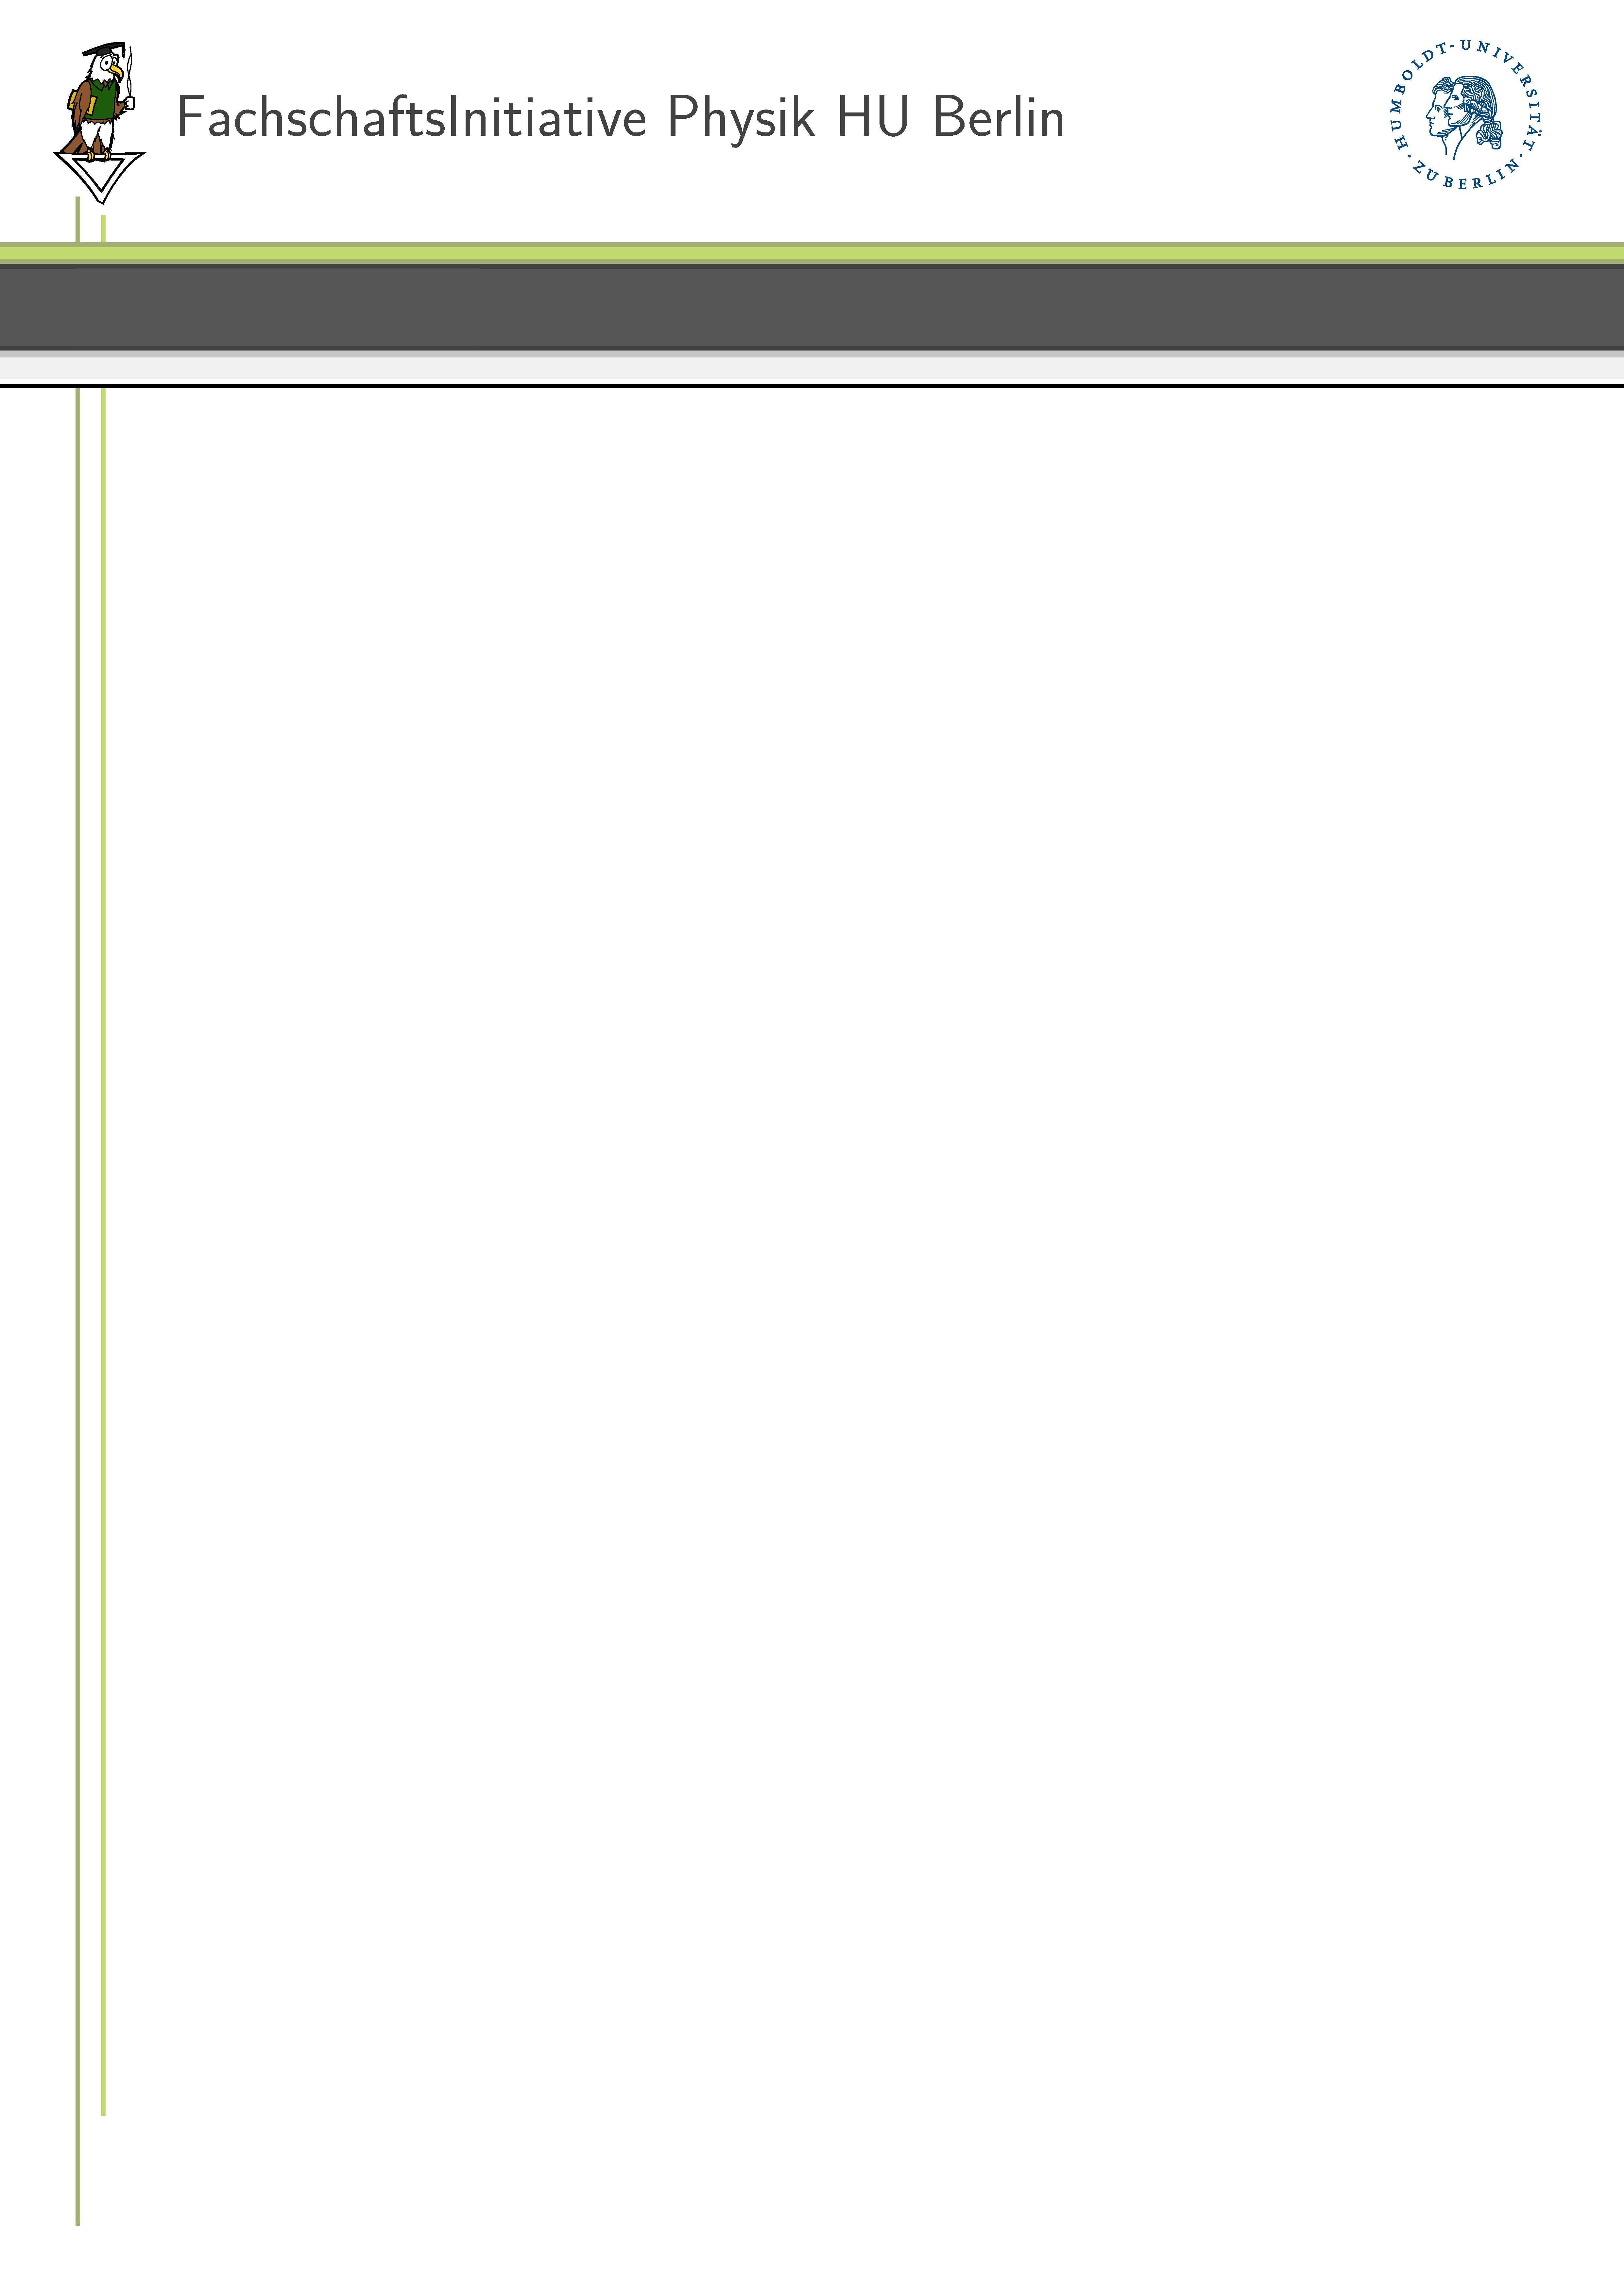
\includegraphics[width=\paperwidth,height=\paperheight,
keepaspectratio]{hintergrund-temp-plain.pdf}
\vfill
}}}

\makeatother

\pagestyle{fancy}
\lfoot{Humboldt-Universität zu Berlin}
\rfoot{\event}

\begin{document}
	\begin{titlepage}
		\AddToShipoutPicture*{\BackgroundPic}
		\begin{center}
			\Large{
			\textcolor{white}{\\\vspace{-2mm}
			\event \\ \textbf{\lecturename}}} \\
			\vspace{15mm}
		\authorname \\
			\vspace{5mm}
		\datum
		\end{center}
		\vspace{1cm}
		\tableofcontents
		\thispagestyle{empty}
	\end{titlepage}
	\ClearShipoutPicture
	
\section{Einführung}

\subsection{Einleitung und Motivation}
"Die Physik ist eine quantifizierende Naturwissenschaft." Das sind die Worte, mit denen Siegfried Großmann \cite{1} seinen Lehrbuch \textit{Mathematischer Einführungskurs für die Physik} einleitet. Der Grund, warum die Physik sowohl im Studium als auch später im Berufsleben so eng mit der Mathematik verbunden ist, ist auch dieser; die Physik versucht, Vorgänge in der Natur für den menschlichen Verstand fassbar zu machen und sie erreicht das durch mathematische Gerüste, die in der Lage sind solche Prozesse zu quantifizieren. Mithilfe solcher Gerüste sind Physiker dann dazu in der Lage, physikalische Begriffe formell zu definieren, sie zu verstehen und daraus dann präzise Vorhersagen zu treffen, die daraufhin bei anderen Bereichen menschlicher Aktivität eine Anwendung finden können. Ziel der meisten physikalischen Beobachtungen und Experimenten ist somit, ein Naturphänomen in die mathematische Sprache übersetzen und dabei auf einer solchen Weise niederschreiben zu können, dass bereits an der grammatikalischen Struktur der Formel eine Aussage über das beschriebene Naturphänomen zu erkennen ist. \\ \\ Um solche mathematische Übersetzungen effektiv auf beobachtbare Vorgänge in unserer Umwelt anwenden zu können, gibt es eine breite Menge an Werkzeugen und Vorgehensweisen in der Mathematik, so wie Taylor-Reihen oder Statistiken. Im Rahmen dieser Vorlesung wollen wir uns aber ganz spezifisch auf einen Werkzeug konzentrieren, der besonders viel Anwendung im Bereich der mathematischen Modellierung von Naturgesetzen findet; nämlich Differentialgleichungen. Differentialgleichungen dienen dazu, das Änderungsverhalten miteinander verknüpfter Größen in der Natur mathematisch darzustellen und einen ersten Ansatz für die Erstellung einer passenden, mathematischen Funktion zu setzen. Sie ermöglichen es also, gewöhnliche Gleichungen für Vorgänge zu finden, bei denen die betrachteten Größen nicht voneinander unabhängig sind, so wie bei der Geschwindigkeit $v$ und der Beschleunigung $a$ in der klassischen Mechanik. \\ \\ Ein passender Beispiel hierzu ist die Fallbewegung einer Kugel unter Berücksichtigung der stokeschen Reibungskraft mit der Luft. Wir gehen nun vom bekannten 2. newtonschen Axiom $F=ma$ aus. Die Beschleunigung $a(t)$, die ein Körper erfährt, ist somit direkt proportional zu der auf ihn wirkenden Kraft $F$. Weiterhin definieren wir; 
\begin{equation}\label{eq1} s(t)=x \ \ \ v(t)=\frac{d}{dt}x=\dot{x} \ \ \ a(t)=\frac{d^2}{dt^2}x=\ddot{x} \end{equation} Ohne die Reibung mit der Luft zu berücksichtigen wäre die einzige Kraft, die auf die Kugel während dem freien Fall wirken würde, die Gravitationskraft der Erde $F_g=-mg$. Somit ließe sich die mathematische Formulierung der Beschleunigung unserer Kugel ganz simpel als 
\begin{equation}\label{eq2} m\ddot{x}=-mg \ \ \Leftrightarrow \ \ \ddot{x}=-g \end{equation} mithilfe der Fallkonstante $g\approx 9,81 \frac{m}{s^2}$ schreiben. Diese Formulierung kann dann durch einfache und doppelte Integration nach der Zeit $t$ jeweils auf Gleichungen der Geschwidigkeit und des Ortes 
\begin{equation}\label{eq3} \dot{x}=-gt+v_o \ \ \ x=-\frac{1}{2}gt^2+tv_0+s_0 \end{equation} ohne weiteres zurückgeführt werden. 
\newpage 
Unter Berücksichtigung der für niedrige Geschwindigkeiten vereinfachbaren, stokeschen Reibungskraft $F_{R}=\beta \dot{x}$ sieht die obige Formel (2) jedoch anders aus, mit \begin{equation}\label{eq4} m\ddot{x}=-mg+\beta \dot{x} \ \ \Leftrightarrow \ \ \ddot{x}=-g+\frac{\beta}{m}\dot{x} \end{equation} wobei $\dot{x}$ nach wie vor die Geschwindigkeit, $m$ die Masse der fallenden Kugel und $\beta$ den Reibungskoeffizient mit der Luft bezeichnet. Da die stokesche Reibungskraft $F_R$ von der Geschwindigkeit $\dot{x}$ abhängt und die Beschleunigung $\ddot{x}$ nichts weiteres ist, als die erste zeitliche Ableitung $\frac{d}{dt}$ von eben dieser Geschwindigkeit, lässt sich diese Differentialgleichung nun nicht mehr einfach durch Integration auf eine Gleichung des Ortes lösen, da die beiden Variablen $\dot{x}$ und $\ddot{x}$ voneinander abhängen. Dies ist in der Physik auch mit mehreren Naturvorgängen der Fall; die Lorentzkraft hängt mit $F_L=q \cdot \dot{\vec{x}} \times \vec{B}$ direkt von der Geschwindigkeit $\dot{\vec{x}}$ des bewegten Teilchens im Magnetfeld ab, beschleunigt aber dann diesen auch mit einer von der Geschwindigkeit abhängigen Beschleunigung $\ddot{\vec{x}}=\frac{q}{m} \cdot \dot{\vec{x}} \times \vec{B}$. Um solche Prozesse mathematisch ausdrücken und quantifizieren zu können ist somit der Umgang mit Differentialgleichungen wie diesen notwendig. 
\subsection{Definition und Klassifizierung}
\subsubsection{Definition}
Die formale Definition von Differentialgleichungen lautet wie folgt;

\begin{center}
\fbox{\parbox{14cm}{\begin{definition}{\textbf{(\textit{Differentialgleichung \cite{2}})}} \\ Eine Gleichung, welche eine (unbekannte) Funktion $f(x)$ und Ableitungen $f^n(x)$ der Funktion bis zur n-ten Ordnung enthält, wird Differentialgleichung (DGL) n-ter Ordnung genannt.\end{definition}}}
\end{center}
Differentialgleichungen sind im allg. also Gleichungen, die aus den Ableitungen einer Funktion sowie aus der gesuchten Funktion selbst bestehen können. Lösung der Differentialgleichung (DGL) sind dann alle Funktionen $f(x)$ die die DGL erfüllen. \\ \\ Eine Differentialgleichung kann somit mehrere Lösungen haben und bei bestimmten Lösungen ist es sogar möglich, einige ihrer Parameter frei zu wählen ohne das dadurch die DGL nicht mehr von der lösenden Gleichung erfüllt wird. Nicht alle Differentialgleichungen sind jedoch analytisch lösbar und bei besonderen Fällen ist sogar mit nummerischen Methoden nur eine annähernde Lösung der DGL möglich. (Weiteres hierzu wird im Laufe des Studiums und nach etwas längerer Auseinandersetzung mit Programmen wie Mathematica behandelt werden) 
\subsubsection{Klassifizierung}
Je nach der Form und Gliederung einer Differentialgleichung kann es unter Umständen angemessen sein, ein bestimmtes Lösungsweg zu wählen oder ein anderes. Im Vergleich zu normalen Gleichungen, die sich während der Schulzeit fast immer durch auflösen nach einer Variable oder in bestimmten Ausnahmefällen mithilfe von Methoden wie der Polynomdivision lösen lassen, sind Differentialgleichungen wie bereits erwähnt nicht immer mit der selben Methode oder sogar überhaupt den gleichen Leitgedanken lösbar. \textit{Für unterschiedliche Klassen von DGLs gibt es unterschiedliche Lösungswege}. Um nun zu wissen, welchen Lösungsweg man für eine bestimmte Differentialgleichung wählen muss, ist es angemessen die Differentialgleichungen nach bestimmten Maßstäben zu \textbf{klassifizieren}. Diese sind;
\begin{flushleft}
\begin{tabular}[h]{l|p{9.6cm}r}

Ordnung der Differentialgleichung & Die Ordnung einer Differentialgleichung, welche eine unbekannte Funktion f(x) enthält, ist die höchste Ableitung $n$ dieser Funktion $f^n(x)$, die in der DGL enthalten ist. Wenn bei einer DGL also z.B. höchstens die n-te Ableitung $f^{(n)}(x)$ der gesuchten Funktion auftritt, handelt es sich um einer \textit{Differentialgleichung n-ter Ordnung}\\ \\ \cline{1-2}
\\ gewöhnlich/partielle DGL & Differentialgleichungen mit einer unbekannten Funktion $f(x)$, in denen Ableitungen der Funktion nach genau einer Variablen $x$ auftreten, nennt man \textit{gewöhnliche Differentialgleichungen}. Wenn eine gesuchte Funktion $f(x,y)$ in der DGL von mehreren Variablen abhängt und die DGL partielle Ableitungen (vgl. VL Differenzieren) nach eben mehreren Variablen $x$ und $y$ enthält, dann ist die Differentialgleichung \textit{partiell}.\\ \\ \cline{1-2}
\\ lineare/nichtlineare DGL & Differentialgleichungen werden linear genannt, wenn die gesuchte Funktion $f(x)$ sowie ihre Ableitungen $f^n(x)$ nur in erster Potenz auftreten und weder im Produkt oder Quotient untereinander noch im Argument einer anderen Funktion stehen. Auch dürfen verschiedengradige Ableitungen der selben Funktion nicht im Produkt miteinander stehen. Nur wenn all diese Kriterien gelten spricht man von einer \textit{linearen Differentialgleichung}. Andernsfalls handelt es sich um einer \textit{nichtlinearen Differentialgleichung}.\\ \\ \cline{1-2}
\\ konstante/nicht konstante Koeffizienten & Bei einer Differentialgleichung kann eine gesuchte Funktion $f(x)$ oder dessen Ableitungen $f^n(x)$ mit einem Koeffizienten $a_i$ versehen sein. Wenn dieser Koeffizient unabhängig von der Variable $x$ der Funktion ist, dann handelt es sich um einen \textit{konstanten Koeffizienten} $a_i$. Hängt $a_i(x)$ aber ebenfalls von $x$ ab, ohne selbst auch die Funktion oder eine Ableitung der Funktion zu sein, dann spricht man von einem \textit{nicht konstanten Koeffizienten}.\\ \\ \cline{1-2}
\\ homogene/inhomogene DGL & Wenn bei einer Differentialgleichung nur Terme auftreten, die zur gesuchten Funktion $f(x)$ und dessen Ableitungen $f^n(x)$ gehören, dann bezeichnet man diese als eine \textit{homogene Differentialgleichung}. Tritt aber zusätzlich zu diesen beiden Arten von Termen in der DGL eine Funktion auf, die entweder konstant oder von der Variablen $x$ abhängt und keine Ableitung der gesuchten Funktion oder die gesuchte Funktion selbst ist, dann handelt es sich um eine \textit{inhomogene Differentialgleichung}. Der ''störende'' Term wird dann dementsprechend als Störfunktion $h(x)$ bezeichnet.\\ \\
\end{tabular}
\end{flushleft}
\subsubsection{Beispiele}
\begin{example}{\textit{Allgemeines Beispiel einer Differentialgleichung}}
\begin{equation}\label{eq5}
a_n \cdot f^{(n)}(x)+a_{n-1}\cdot f^{(n-1)}(x)+...+ a_0 \cdot f(x)=h(x)
\end{equation}
Um Differentialgleichungen klassifizieren zu können kann es zuerst angemessen sein, sie in der Form einer Folge der einzelnen Ableitungen in absteigender Reihenfolge von links nach rechts darzustellen. Dabei bezeichnet $f^{(n)}(x)$ die n-te Ableitung der gesuchten Funktion $f(x)$, weshalb auch $f^{(0)}(x)=f(x)$ gilt. Die Faktoren $a_0, a_1, a_2,...,a_n$ sind die Koeffizienten. Als Summe lässt sich diese Folge auch ganz prägnant umschreiben als;
\begin{equation}\label{eq5}
\sum_{k=0}^n a_k f^{(k)}(x)=h(x)
\end{equation}
Anhand von diesen Beispiel kann man auch gut erklären, auf welche stellen man mit der Klassifizierung hinzuschauen hat. Das höchste n-Glied markiert hier z.B. die Ordnung der Differentialgleichung, die Koeffizienten $a_n$ bis $a_0$ sind je nach Abhängigkeit von der Variablen $x$ als konstant oder nicht konstant einzustufen und je nachdem, ob die Störfunktion $h(x)$ nicht Null ist, kann die DGL als homogen oder inhomogen klassifiziert werden.
\end{example}
\vspace{0,5cm}
\begin{example}{\textit{Freier Fall}}
\\ Ein sehr einfacher Beispiel für eine Differentialgleichung, der auch u.U. als triviale DGL bezeichnet werden kann, ist der freie Fall unter dem Einfluss des Gravitationsfeldes der Erde und ohne die Luftreibung miteinzubeziehen. Wie bereits in der Einleitung erläutert lässt sich diese DGL schreiben als 
\begin{equation}
m\ddot{x}=-mg \ \ \Leftrightarrow \ \ \ddot{x}=-g
\end{equation}
Hierbei handelt es sich also um eine gewöhnliche, inhomogene Differentialgleichung zweiter Ordnung ohne Koeffizienten (Die Störfunktion $h(x)$ ist hierbei mit der Fallbeschleunigung $g(t)=g$ als zeitlich konstant anzusehen). Bei den meisten Fällen wäre eine solche DGL etwas umständlicher zu lösen, doch bei diesen ist es aufgrund des einmaligen Auftretens der gesuchten Funktion, hier in der zweiten Ableitung, viel einfacher. Integrieren auf beiden Seiten liefert;
\begin{equation}
\int \ddot{x} dt=\int -g dt
\end{equation}
\begin{equation}
\dot{x}=-gt+v_0
\end{equation}
\begin{equation}
\int \dot{x} dt=\int -gt+v_0 dt
\end{equation}
\begin{equation}
x=-\frac{1}{2} gt^2+v_0t+x_0
\end{equation}
\end{example}
\vspace{0,5cm}
\begin{example}{\textit{Lorentzkraft}}
\\ Auch die Bewegungsgleichung beschleunigter Ladungsträger im Magnetfeld lässt sich, wie bereits in der Einleitung erwähnt, mithilfe einer Differentialgleichung bestimmen. Ein Ladungsträger der Masse $m$, der sich mit einer elektrischen Ladung $q$ und einer Geschwindigkeit $\dot{\vec{x}}$ in einem magnetischen Feld der magnetischen Feldstärke $\vec{B}$ bewegt, wird wie folgt beschleunigt;
\begin{equation}
m\ddot{\vec{x}}=q \cdot \dot{\vec{x}} \times \vec{B}
\end{equation}
\begin{equation}
\ddot{\vec{x}}=\frac{q}{m} \cdot \dot{\vec{x}} \times \vec{B}
\end{equation}
Es handelt sich hierbei also um eine gewöhnliche, homogene Differentialgleichung zweiter Ordnung mit konstanten Koeffizienten (letzteres je nachdem ob die magnetische Feldstärke $\vec{B}$ und die Ladung $q$ als zeitlich konstant angenommen werden oder nicht). \\ \\ Da die gesuchte Funktion nun bereits zweimal in der DGL vorkommt, einmal in seiner ersten und einmal in seiner zweiten Ableitung, ist diese auch wiederum nicht mehr bloß trivial zu lösen, kann aber durch geeignetes wählen eines Lösungsansatzes relativ einfach geklärt werden. Dieser Beispiel wird später während der Übungen zu den Lösungsansätzen noch einmal aufgegriffen werden. 
\end{example}
\vspace{0,5cm}
\begin{example}{\textit{Inhomogene, nichtlineare und partielle Differentialgleichungen}}
\\ Wie bereits erläutert müssen nicht alle Differentialgleichungen eine analytische oder sogar eine nummerische (d.h. mit algebraischen Programmen angenäherte) Lösung besitzen.
\begin{center}
\begin{minipage}{.5\textwidth}
  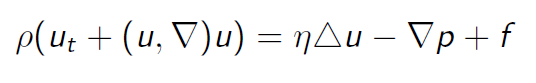
\includegraphics[width=0.9\linewidth]{navierstokes.png}
\\  \caption{Abb.1- Navier-Stokes Gleichung}
\end{minipage} 
\end{center}
\\ \\ Die Navier-Stokes Gleichungen, die die Strömung von linear-viskosen Flüssigkeiten unter Berücksichtigung der Reibung zwischen den Teilchen der strömenden Flüssigkeit beschreiben, sind bspw. ein System von nichtlinearen partiellen Differentialgleichungen zweiter Ordnung die bis zum heutigen Tag keine einheitliche Lösung haben. Dies kann bei Differentialgleichungen vor allem dann der Fall sein, wenn diese inhomogen, partiell und/oder nichtlinear sind. Solche DGLs können unter Umständen zwar auch gelöst werden (vgl. VL DGL.2), jedoch sind die angewandten Lösungsansätze viel mehr von der jeweiligen DGL und dessen Struktur abhängig. \\ \\
Weitere Differentialgleichungen dieser Art, die wir zwar nicht lösen aber klassifizieren werden, sind; 
\begin{equation}
\frac{d}{dt}\left(\frac{\partial L}{\partial \dot{\varphi}}\right)}-\frac{\partial L}{\partial \varphi}=0
\end{equation}
Lineare, partielle, homogene Differentialgleichung 1.Ordnung, mit $L=L(\varphi, \dot{\varphi},t)$
\begin{equation}
sin(\ddot{f})^2+\frac{8x}{e^{\dot{f}}}-cos(x)f=16x^2
\end{equation}
Nichtlineare, gewöhnliche, inhomogene Differentialgleichung 2.Ordnung mit nicht konstanten Koeffizienten und $f=f(x)$
\begin{equation}
\varphi^{(4)}(t)\cdot \varphi^{(2)}(t)+8\varphi(t)=sin(t)
\end{equation}
Nichtlineare, gewöhnliche, inhomogene Differentialgleichung 2.Ordnung mit konstanten Koeffizienten und $\varphi=\varphi(t)$
\end{example}
\\ \\
\newpage
\section{Homogene Differentialgleichungen}

\subsection{Allgemeine Lösung}
Eine Funktion $f(x)$, für die man ein oder mehrere Parameter $c_n$ frei wählen kann ohne das die Funktion dadurch die DGL nicht mehr erfüllt, heißt allgemeine Lösung der Differentialgleichung. Wenn eins oder alle Parameter der allgemeinen Lösung festgesetzt sind, dann wird diese als spezielle Lösung der Differentialgleichung bezeichnet. Formell definiert man;
\begin{center}
\begin{flushleft}
\rule{8cm}{0,01cm}
\end{flushleft}
\begin{sentence}{\textbf{(\textit{Allgemeine Lösung \cite{2}})}} \\ Die allgemeine Lösung einer DGL n-ter Ordnung enthält genau $n$ Integrationskonstanten $c_n$. Zudem beinhaltet sie jede spezielle Lösung. Für Differentialgleichungen, die mit dem Exponentialansatz (Satz 2.3) lösbar sind, gilt zusätzlich;
\begin{equation}
f(x)=C_1\cdot e^{\lambda _1x}+...+C_n\cdot e^{\lambda _nx}
\end{equation}
\begin{center}
bzw.
\end{center}
\begin{equation}
f(x)=\sum_{k=0}^n C_k\cdot e^{\lambda _kx}
\end{equation}
mit $C_k$ als Integrationskonstanten und $\lambda_k$ als mögliche Lösungen des charakteristischen Polynoms 
\end{sentence}
\begin{flushleft}
\rule{8cm}{0,01cm}
\end{flushleft}
\end{center}
Ziel bei der Lösung einer Differentialgleichung ist also, insofern dies möglich ist die allgemeine Lösung zu bestimmen um daraus dann durch gezieltes wählen der Parameter $C_n$ die spezielle Lösung nach Bedarf herleiten zu können. (vgl. VL DGL.2)
\subsection{Lösungsansätze}

\subsubsection{Separation der Variablen}
Der erste Lösungsansatz, mit dem wir uns beschäftigen werden, ist die Separation der Variablen. Dieser beruht auf der folgenden Gleichheit aus dem Bereich der Differentiation;
\begin{equation}
\frac{d}{dx}f(x)=f'(x)
\end{equation}
Formell kann er nach dem folgenden Satz benutzt werden
\begin{center}
\begin{flushleft}
\rule{8cm}{0,01cm}
\end{flushleft}
\begin{sentence}{\textbf{(\textit{Separation der Variablen \cite{2}})}} \\
Eine Differentialgleichung, welche sich in der Form 
\begin{equation}
f'(x)=g(f(x))\cdot h(x)
\end{equation}
schreiben lässt, kann durch das Verfahren \textit{Separation der Variablen} gelöst werden. Dabei ist $f(x)$ die gesuchte Funktion
\end{sentence}
\begin{flushleft}
\rule{8cm}{0,01cm}
\end{flushleft}
\end{center}
Dieser Ansatz kann also nur bei homogenen Differentialgleichungen angewendet werden, die sich in einer Form umschreiben lassen bei der die erste Ableitung $f'(x)$ der gesuchten Funktion alleine auf einer Seite steht und die normale Funktion auf der andere (wobei die normale Funktion $f(x)$ nicht unbedingt alleine, sondern auch innerhalb einer anderen Funktion $g(f)$ oder zusammen mit einem nichtkonstanten Koeffizienten $h(x)$ sein darf.)\\ \\ 
\begin{guide}{\textbf{(\textit{Verfahren})}} \\
Zuerst muss die homogene Differentialgleichung in die Form 
\begin{equation}
f'(x)=g(f(x))\cdot h(x)
\end{equation}
gebracht werden (Satz 2.2). Sobald die DGL in dieser Form steht, setzen wir die Gleichheit (19) aus der Differentiation 
\begin{equation}
\frac{df}{dx}=f'(x)
\end{equation}
in die DGL ein, s.d. nun steht;
\begin{equation}
\frac{df}{dx}=g(f(x))\cdot h(x)
\end{equation}
Nun wollen wir etwas machen, was in der formalen Mathematik oft unbeliebt ist (Da $df$ und $dx$ infinitesimale und keine Zahlen sind, mit denen man formal rechnen sollte). Wir multiplizieren die ganze DGL mit $dx$, damit dieser in der Gleichung alleine mit dem $h(x)$ auf einer Seite übrig bleibt und das $df$ zusammen mit dem $g(f(h))$ auf der anderen. Es ist auch wichtig, dass das $df$ und das $dx$ im Zähler stehen (also nicht teilen), damit wir später integrieren können. Es sollte nun allg. stehen;
\begin{equation}
\frac{1}{g(f(x))}df=h(x)dx
\end{equation}
Integration beider Seiten liefert dann
\begin{equation}
\int \frac{1}{g(f(x))}df= \int h(x)dx
\end{equation}
sowie eine Integrationskonstante $c_i$ an den beiden aufgeleiteten Termen. Ab diesen Punkt hängt das weitere Verfahren vom Ergebnis der Integration für die jeweilige DGL ab. Da durch die Separation der Variablen die Ableitung der gesuchten Funktion nicht mehr in der DGL steht, sollte diese ab dieser Stelle auch durch gewöhnliches umformen lösbar sein. Anhand eines Beispieles wird dieses Verfahren jedoch zur Übersicht kurz nochmals geschildert werden, bevor wir zum Exponentialansatz fortfahren. 
\end{guide}
\vspace{0,5cm}
\begin{example}{\textit{Lösung durch Separation der Variablen}} \\ \\
Es sei folgende Differentialgleichung gegeben
\begin{equation}
\frac{2xf(x)^2}{f'(x)}=1
\end{equation}
Umformen nach (21)
\begin{equation}
2xf(x)^2=f'(x)
\end{equation}
Trennen der Variablen (23)
\begin{equation}
2xf(x)^2=\frac{df}{dx}
\end{equation}
Umformen nach (24) um später zu integrieren
\begin{equation}
2xdx=\frac{1}{f(x)^2}df
\end{equation}
Beidseitiges integrieren nach (25)
\begin{equation}
x^2+c_i=-\frac{1}{f(x)}+c_k
\end{equation}
Umformen nach $f(x)$ mit $C=c_i-c_k$
\begin{equation}
f(x)=-\frac{1}{x^2+C}
\end{equation}
\subsubsection{Exponentialansatz}
Der Exponentialansatz baut, wie sein Name auch schon verrät, auf der Exponentialfunktion Eulers auf. Sie geht von der Aussage aus, dass die Funktion, die die Differentialgleichung lösen kann, als eine e-Funktion der Form $f(x)=\sum_{k=0}^n C_k\cdot e^{\lambda _kx}$ dargestellt werden kann. Auch hier gibt es einen formalen Satz für die Anwendung des Ansatzes;
\begin{center}
\begin{flushleft}
\rule{8cm}{0,01cm}
\end{flushleft}
\begin{sentence}{\textbf{(\textit{Exponentialansatz \cite{2}})}} \\
Eine homogene lineare Differentialgleichung mit konstanten Koeffizienten lässt sich mit dem Exponentialansatz lösen. Dieser besagt, dass die gesuchte Funktion eine Linearkombination aus Termen der Form $f(x)=C\cdot e^{\lambda x}$ besteht.
\end{sentence}
\begin{flushleft}
\rule{8cm}{0,01cm}
\end{flushleft}
\end{center}
Dieser Ansatz geht also von der Annahme aus, dass die gesuchte Funktion für unsere DGL in der Form $f(x)=\sum_{k=0}^n C_k\cdot e^{\lambda _kx}$ geschrieben werden kann. Dass diese Annahme richtig für beliebige, lineare und homogene DGLs mit konstanten Koeffizienten ist, wird später ausführlich während dem Studium behandelt. \\ \\ $C_k$ und $\lambda$ seien nun unbestimmte komplexe Zahlen $C$ der Exponentialfunktion, die wenn richtig ausgewählt, die DGL erfüllen können. Für die allgemeine Lösung der DGL sind jedoch nur die Konstanten $\lambda_k$ vonnöten. Die Bedeutung von der Konstanten C wird später bei der Vorlesung für DGL.2 näher betrachtet werden. \\ \\
\begin{guide}{\textbf{(\textit{Verfahren})}} \\
Gegeben sei eine beliebige, lineare, homogene Differentialgleichung n-ter Ordnung in seiner allgemeinen Form und mit konstanten Koeffizienten $a_n$,$a_{n-1}$,..., $a$;
\begin{equation}
a_n\cdot f^{(n)}(x)+a_{(n-1)}\cdot f^{(n-1)}(x)+...+a\cdot f(x)=0
\end{equation}
Da diese Differentialgleichung alle Bedingungen erfüllt (homogenität, linearität, konst. Koeffiz.), kann der Exponentialansatz angewendet werden. Der erste Schritt, um mit dem Ansatz anzufangen, ist diesen nun in die Funktion einzusetzen. Hierfür bilden wir alle Ableitungen der Exponentialfunktion bis zur Ordnung unserer DGL (hier also bis zur n-ten Ordnung) damit wir diese dann in die DGL einsetzen können. Wir bilden somit;
\begin{equation}
f(x)=C\cdot e^{\lambda x}
\end{equation}
\begin{equation}
(...)
\end{equation}
\begin{equation}
f^{(n-1)}(x)=\lambda^{n-1} \cdot C\cdot e^{\lambda x}
\end{equation}
\begin{equation}
f^{(n)}(x)=\lambda^n \cdot C\cdot e^{\lambda x}
\end{equation}
Eingesetzt in die DGL kriegen wir die Folge
\begin{equation}
\Rightarrow a_n \cdot \lambda^n \cdot C\cdot e^{\lambda x}+a_{n-1} \cdot \lambda^{n-1} \cdot C\cdot e^{\lambda x}+...+a\cdot C\cdot e^{\lambda x}=0
\end{equation}
was dann durch ausklammern weiter vereinfacht werden kann auf;
\begin{equation}
(a_n \cdot \lambda^n+a_{n-1} \cdot \lambda^{n-1}+...+a) \cdot C\cdot e^{\lambda x}=0
\end{equation}
Man sieht, da die Konstante $C$ keine $0$ sein darf und die Exponentialfunktion $e^{\lambda x}$ für beliebige Werte von $x$ nie Null wird, dass die innere Funktion
\begin{equation}
a_n \cdot \lambda^n+a_{n-1} \cdot \lambda^{n-1}+...+a=0
\end{equation}
Null ergeben muss, damit die DGL unter diesen Ansatz erfüllt wird. Dies ist das sogenannte \textit{charakteristische Polynom}. Somit können wir auch anhand von den Nullstellen dieses Polynoms die zugehörigen Werte für $\lambda_n$ ausrechnen und diese dann in die Exponentialfunktion einsetzen. Da es sich um einen Polynom n-ten Grades handelt müssten hier für $\lambda_n$ außerdem genau n Werte existieren, bei Polynomen höheren Grades können aber auch noch weitere Werte für $\lambda$ vorkommen. Als Endergebnis soll allgemein zustande kommen;
\begin{equation}
f(x)=C_1\cdot e^{\lambda_1 x}+C_2\cdot e^{\lambda_2 x}+...+C_n\cdot e^{\lambda_n x}
\end{equation}
\vspace{0,5cm}
\begin{example}{\textit{Lösung durch Exponentialansatz}} \\ \\
Es sei folgende Differentialgleichung gegeben
\begin{equation}
4\ddot{x}-x=-2\dot{x}
\end{equation}
Umformen nach (32)
\begin{equation}
4\ddot{x}+2\dot{x}-x=0
\end{equation}
Aufstellen der vermeintlichen Exponentialfunktion und dessen Ableitungen (33-36)
\begin{equation}
x(t)=C\cdot e^{\lambda t}
\end{equation}
\begin{equation}
\dot{x}(t)=\lambda \cdot C\cdot e^{\lambda t}
\end{equation}
\begin{equation}
\ddot{x}(t)=\lambda^2 \cdot C\cdot e^{\lambda t}
\end{equation}
Einsetzen der e-Funktion und dessen Ableitungen in die DGL (36)
\begin{equation}
4\lambda^2 \cdot C\cdot e^{\lambda t}+2\lambda \cdot C\cdot e^{\lambda t}-C\cdot e^{\lambda t}=0
\end{equation}
Ausklammern und aufstellen des charakteristischen Polynoms (37)
\begin{equation}
(4\lambda^2+2\lambda-1)C\cdot e^{\lambda t}=0
\end{equation}
Ausrechnen der Nullstellen des charakteristischen Polynoms (38) und Bestimmung der $\lambda_n$
\begin{equation}
4\lambda^2+2\lambda-1=0
\end{equation}
\begin{equation}
(2\lambda+\frac{1}{2})^2-\frac{5}{4}=0
\end{equation}
\begin{equation}
(2\lambda+\frac{1}{2})^2=\frac{5}{4}
\end{equation}
\begin{equation}
2\lambda+\frac{1}{2}=\pm \sqrt{\frac{5}{4}}
\end{equation}
\begin{equation}
\lambda_{1/2}=\frac{\pm \sqrt{\frac{5}{4}}-\frac{1}{2}}{2}
\end{equation}
Einsetzen von $\lambda_{1/2}$ in die Exponentialfunktion gemäß (39)
\begin{equation}
x(t)=C_1\cdot e^{\frac{\sqrt{5}-1}{4}t}+C_2\cdot e^{\frac{-\sqrt{5}-1}{4}t}
\end{equation}
\begin{thebibliography}{1}
		%\bibitem{label}AUTHOR: TITLE, PUBLISHER, YEAR
		\bibitem{1} Prof. Dr. Siegfried Großmann: \textit{Mathematischer Einführungskurs für die Physik}, 2012
		\bibitem{2} Katharina Melisande Albrecht, Thomas Guy Rauch: \textit{Differentialgleichungen-Vorlesungsskript Brückenkurs 2018/2019}
		\bibitem{3} Walter Winter: \textit{Vorlesungsskript-Mathematische Grundlagen, WiSe 2018/2019}
	\end{thebibliography}
	
\end{document}